%%%%%%%%%%%%%%%%%%%%%%%%%%%%%%%%%%%%%%%%%%%%%%%%%%%%%%%%%%%%%%%%%%%
%                                                                 %
%                            APPENDICES                           %
%                                                                 %
%%%%%%%%%%%%%%%%%%%%%%%%%%%%%%%%%%%%%%%%%%%%%%%%%%%%%%%%%%%%%%%%%%%

\appendix    % This command is used only once!
%\addcontentsline{toc}{chapter}{APPENDICES}             %toc entry  or:
\addtocontents{toc}{\parindent0pt\vskip12pt APPENDICES} %toc entry, no page #

\chapter{Key Algorithms}

\section{Array Primitives}

\subsection{Immutable Arrays}

\subsection{Reduction}

\subsection{Scan}

\subsection{Sort}

\chapter{Topological Ratios}

\section{Maximum Upward Adjacencies}

\subsection{From Vertices}
\label{app:vert_up_deg}

We begin by proving an upper bound on tetrahedra sharing a vertex,
which must be based on some assumed geometric restriction,
because topology alone does not dictate any such bound.
We will begin with the most straightforward restriction, that
of solid angles, and correlate it to the mean ratio quality measure
defined by Equation \ref{eq:tet_mean_ratio} from Section \ref{sec:def_quality}.

Each tetrahedron adjacent to a vertex forms a solid angle at
the corner where the adjacency occurs.
For a given vertex, the sum of these solid angles for all
adjacent tetrahedra cannot exceed $4\pi$, the solid angle of a sphere.
Conversely, if there are $n$ tetrahedra adjacent to one vertex,
then one or more of the tetrahedra will satisfy Inequality
\ref{eq:solid_angle_degree}, where $\mathbf{\Omega}$ is the
solid angle of the relevant corner.

We assume that the way to maximize the mean ratio of a tetrahedron
that has one solid angle equal to $\mathbf{\Omega}$ is to have
its other three corners form an equilateral triangle.

Since the mean ratio is scale-invariant, we can consider this
without loss of generality for a tetrahedron $(o,a,b,c)$ where
$o$ is the center of a unit sphere and $(a,b,c)$ are on the surface
of that sphere, and form an equilateral triangle
as shown in Figure \ref{fig:solid_angle}.
Let $\theta$ be the angle $\angle oab = \angle obc = \angle oca$,
Intuitively, as $\theta$ increases from zero to $\frac23\pi$,
the solid angle $\mathbf{\Omega}$ at $o$ monotonically
increases from zero to $2\pi$.
The exact relation between $\mathbf{\Omega}$ and $\theta$ is given by Equation
\ref{eq:solid2side}
using an intermediate $\phi$ (the dihedral angle between any pair of triangular
faces meeting at $o$).

\begin{figure}
\begin{center}
\includegraphics[width=0.4\textwidth]{solid_angle.png}
\caption{Maximizing quality versus solid angle}
\label{fig:solid_angle}
\end{center}
\end{figure}

\begin{equation} \label{eq:solid_angle_degree}
\mathbf{\Omega} \leq \frac{4\pi}{n}
\end{equation}

\begin{gather} \label{eq:solid2side}
\begin{split}
\phi &= \arccos\left(\frac{\cos\theta - \cos^2\theta}{\sin^2\theta}\right) \\
\mathbf{\Omega} &= 3\phi - \pi = 3\arccos\left(\frac{\cos\theta - \cos^2\theta}{\sin^2\theta}\right) - \pi
\end{split}
\end{gather}

Let $l=2\sin\left(\frac{\theta}{2}\right)$ be the length of any cord $(a,b)$, $(b,c)$, or $(c,a)$.
We can use properties of equilateral triangles and isosceles
tetrahedra to derive the mean ratio quality of this tetrahedron
in terms of $l$ as shown in Equation \ref{eq:solid_angle_qual}.
The ranges for valid tetrahedra are $\theta\in[0,\frac23\pi]$ and $l\in[0,\sqrt{3}/2]$,
in which quality varies monotonically with solid angle.

\begin{gather} \label{eq:solid_angle_qual}
\begin{split}
h &= \tfrac{\sqrt{3}}{2}l \\
r &= \tfrac13 h = \tfrac{1}{2\sqrt{3}}l \\
R &= 2r = \tfrac{1}{\sqrt{3}}l \\
A &= \tfrac{\sqrt{3}}{4}l^2 \\
H &= \sqrt{1-R^2} = \sqrt{1-\tfrac13 l^2} \\
V &= \tfrac13 A H = \tfrac{1}{4\sqrt{3}} l^2\sqrt{1-\tfrac13 l^2} \\
l_{\text{MS}} &= \tfrac16(3l^2 + 3) = \tfrac12(l^2 + 1) \\
\eta^3 &= \frac{V^2}{\gamma^2 l_{\text{MS}}^3} =
\frac{2^3}{4^2\cdot 3}\frac{l^4(1-\tfrac13 l^2)}{\gamma^2 (l^2 + 1)^3}
\end{split}
\end{gather}

In conclusion, if we ensure that all tetrahedra in a mesh have
quality $\geq Q_{\text{min}}$, then we also guarantee that no
vertex in the mesh can have more than some $n_{\text{max}}$
tetrahedra adjacent.
We can use the extreme case in Figure \ref{fig:solid_angle}
to plot this relation, as shown in Figure \ref{fig:max_tet_deg}

\begin{figure}
\begin{center}
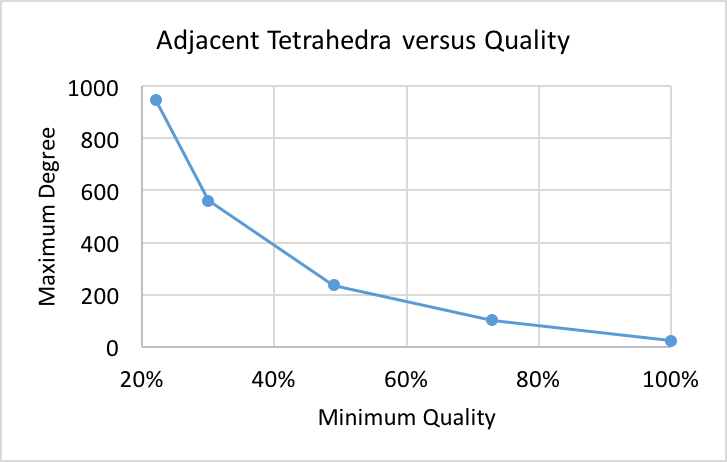
\includegraphics[width=0.6\textwidth]{max_tet_deg.png}
\caption{Maximum vertex-tetrahedron degree given a minimum tetrahedron mean ratio}
\label{fig:max_tet_deg}
\end{center}
\end{figure}

A similar yet much simpler analysis, applied to triangles
from the origin to the edge of a unit circle, results in the
plot given by Figure \ref{fig:max_tri_deg}.

\begin{figure}
\begin{center}
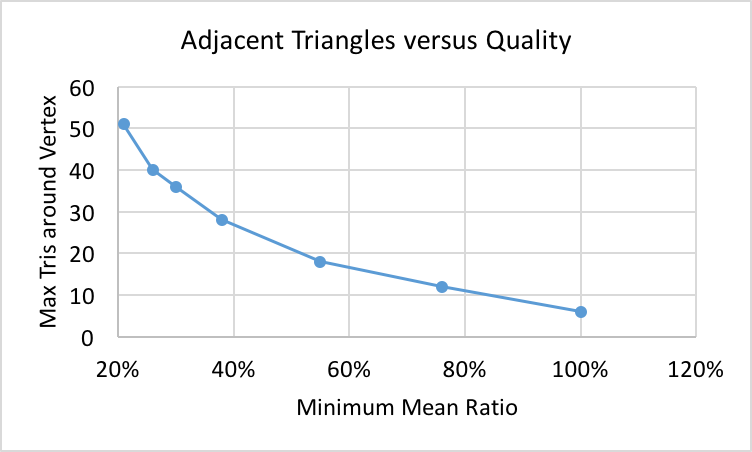
\includegraphics[width=0.6\textwidth]{max_tri_deg.png}
\caption{Maximum vertex-triangle degree given a minimum triangle mean ratio}
\label{fig:max_tri_deg}
\end{center}
\end{figure}
